\documentclass[margin]{res}
\usepackage[icelandic]{babel}
\usepackage[T1]{fontenc}
\usepackage[utf8x]{inputenc}
\usepackage{graphicx}
\usepackage{url}
\setlength{\textwidth}{5.1in}

\begin{document}
\begin{figure}
\begin{minipage}[b]{0.45\linewidth}
\section {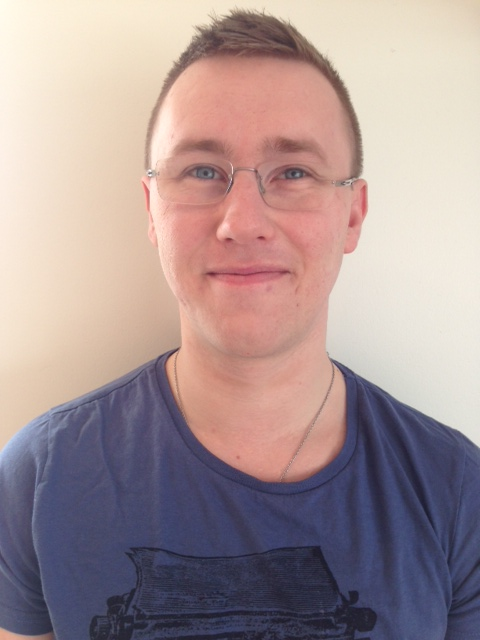
\includegraphics[height=4.8cm]{gberg_profile}}
\end{minipage}
\hspace{0.5cm}
\begin{minipage}[b]{0.45\linewidth}
{\large\bf Guðmundur Berg Hjaltason}\\
 Hólmvaði 8\\
 110, Reykjavík Iceland\\
 gudmberg@gmail.com\\
 Mobile: (+354) 867-5534\\
\end{minipage}
\end{figure}

\begin{resume} 
\section{Um mig}
Fæddur 4. Október 1985, er trúlofaður Guðríði Kristínu Magnúsdóttir og er í sambúð með henni ásamt hundinum okkar.
Ég starfa hjá 365 Miðlum sem Þjónustufulltrúi í tækniveri.

\section{Vinna \& Skóli}
2014: 365 Miðlar ehf \footnote{\url{http://www.365.is}}: \emph{Þjónustufulltrúi Tæknivers.}\\
2010 - 2012: Háskólinn í Reykjavík: \emph{Frumgreinar.}\\
2007 - 2010: Síminn: \footnote{\url{http://www.siminn.is}} \emph{Tæknimaður í Vettvangsþjónustu.}\\
2007: Pizza Hut: \emph{Bakari.}\\
2005 - 2006: Pizzahöllin: \emph{Bakari.}\\
2004: Hólmsteinn Pétursson: \emph{Múrvinna.}

\section{Önnur námskeið}
2014: edx.org: \emph{6.00x Introduction to Computer Science and Programming Using Python.}\footnote{\url{https://www.edx.org/course/mitx/mitx-6-00-1x-introduction-computer-1841\#.U6jCiHVJXUY}} Inngangs námskeið Tölvunafræði hjá MIT\\
\url{https://s3.amazonaws.com/verify.edx.org/downloads/f1e610f209444903a7469c4a8431c33b/Certificate.pdf}\\
2014: edx.org: \emph{cs1.69x Engineering Software as a Service} \footnote {\url{https://www.edx.org/course/uc-berkeleyx/uc-berkeleyx-cs169-1x-engineering-1377\#.U6jB33VJXUY}} Lært Ruby on Rails, Agile hugmyndafræði, TDD, BDD, Git Version Control, SaaS Architecture\\
\url{https://s3.amazonaws.com/verify.edx.org/downloads/c42d3b5d0cb14f4bb8be95c634fd4cba/Certificate.pdf}\\
2011: Promennt: \emph{Comptia A+}\footnote{\url{http://www.promennt.is}} Tölvuviðgerðir og viðhald.\\
2011: NTV: \emph{Alvöru vefsíðugerð.}\footnote{\url{http://www.ntv.is}} Á námskeiðinu var kennt HTML, CSS og ASP\\

\section{Meðmælendur}

Hlynur Sigurþórsson
\begin{itemize}\itemsep -3pt
\item Azazo.is
\item hlysig@gmail.com
\item (+354) 893-1000
\end{itemize}

Svavar Kárason
\begin{itemize}\itemsep -3pt
\item 365 Miðlar
\item svavarkari@365.is
\item (+354) 6969210
\end{itemize}

Óskar Gíslason
\begin{itemize}\itemsep -3pt
\item Fyrrum yfirmaður minn hjá Símanum.
\item vesen@mail.dk
\item (+45) 40198244
\end{itemize}

\section{Hæfileikar} 
{\sl Forritunar Tungumál}: Forritunar tungumál sem ég kann og hef notast við eru
C, Python, Ruby, HTML, CSS og Javascript.

{\sl Stýriskerfi:} Windows, OS X og linux stýrikerfi. Ég nota persónulega sjálfur aðeins osx eða linux.

{\sl Tungumál:} Ég tala/skrifa bæði íslensku og ensku.

{\sl Personal:}
Ég er mjög áhugasamur, með mikinn drifkraft, áreiðanlegur og duglegur. Hef mikinn áhuga á að læra nýja hluti og hef mjög gaman af því.

\section{Áhugamál}
Mestur tími minn fer í tölvutengda hluti. Ég eyði mjög miklum tíma að lesa forritunarbækur, blog
og aðra þræði um forritun og því tengt. Hef mikinn áhuga á fótbolta og íþróttum og er harður Man Utd aðdáandi.

Mér finnst gaman að eyða frítíma mínum að horfa á góðar bíómyndir og sérstaklega fara á flottar sci-fi myndir í bíó.
Ég hef mjög gaman að því að eyða tíma með hundinum mínum og fara í langa göngutúra með henni. 
\end{resume}
\end{document}
